% ECE501 Digital Image Processing -- Week 6 Project Progress Report (Group 15)
% Build: tectonic main.tex
\documentclass[11pt,a4paper]{article}

\usepackage[margin=2.2cm]{geometry}
\usepackage[T1]{fontenc}
\usepackage{lmodern}
\usepackage{microtype}
\usepackage{amsmath,amssymb}
\usepackage{graphicx}
\usepackage{booktabs}
\usepackage{tabularx}
\usepackage{longtable}
\usepackage{array}
\usepackage{multirow}
\usepackage[table]{xcolor}
\usepackage{enumitem}
\usepackage{caption}
\usepackage{fancyhdr}
\usepackage{listings}
\usepackage{tikz}
\usetikzlibrary{positioning,arrows.meta,fit,backgrounds}
\usepackage[colorlinks=true,linkcolor=blue!50!black,citecolor=blue!60!black,urlcolor=blue!60!black]{hyperref}

\definecolor{hdr}{HTML}{DCE6F2}
\definecolor{codebg}{HTML}{F6F8FA}
\definecolor{okgreen}{HTML}{1E7B34}
\definecolor{badred}{HTML}{B3261E}

\newcommand{\code}[1]{\texttt{\detokenize{#1}}}
\newcolumntype{L}{>{\raggedright\arraybackslash}X}
\newcolumntype{C}{>{\centering\arraybackslash}X}
\newcolumntype{R}{>{\raggedleft\arraybackslash}X}

\lstset{
  basicstyle=\ttfamily\footnotesize,
  backgroundcolor=\color{codebg},
  frame=single, rulecolor=\color{black!15},
  breaklines=true, columns=fullflexible,
  keywordstyle=\color{blue!60!black}\bfseries,
  commentstyle=\color{black!55}\itshape,
  stringstyle=\color{okgreen},
  showstringspaces=false,
  xleftmargin=2pt, xrightmargin=2pt
}

\captionsetup{font=small,labelfont=bf}
\setlist{itemsep=2pt,topsep=4pt}
\emergencystretch=3em

\pagestyle{fancy}
\fancyhf{}
\fancyfoot[C]{\small Group 15 \textbar\ Week 6 Project Progress Report \textbar\ Page \thepage}
\renewcommand{\headrulewidth}{0pt}

\begin{document}

\begin{center}
{\LARGE\bfseries Week 6 Project Progress Report}\\[4pt]
{\large\bfseries Adaptive Fabric Surface Defect Detection and Localization using\\ Classical Texture Descriptors}
\end{center}

\noindent
\textbf{Course Name:} ECE501 Digital Image Processing (DIP)\\
\textbf{Group Number:} Group 15\\
\textbf{Group Members:} Rinal Shah, Varun Hotani, Aadi Mehta, Pratik Agrawal\\
\textbf{Week Number:} Week 6\\
\textbf{Date:} October 27, 2026\\
\textbf{Deliverable:} Production directory structure; full AFID benchmark; Gabor descriptor; $64\times64$ refinement; one-class baselines; ablation study\\
\textbf{Branch:} \code{feat/week-6} (merged into \code{main})

\section*{Objectives of the Week}
\begin{itemize}
  \item Reorganise \code{Codes/} into a production layout taken from published conventions: the PyPA \emph{src layout} \cite{pypa} and the \emph{cookiecutter-data-science} module split \cite{ccds}. Each layer (configuration, data, features, modelling, evaluation, pipelines, CLI) gets its own subpackage.
  \item Acquire the full AFID dataset \cite{silvestre2019}, check it, and re-run the benchmark on \emph{all} defective images. This is the first complete real-data evaluation of the project, after the 13-image mid-semester run and the data-less Week~5.
  \item Implement the two remaining descriptor and localization items from the original plan: a Gabor filter bank \cite{jain1991} and a nested $64\times64$ refinement of flagged $256\times256$ windows.
  \item Implement the planned baselines, One-Class SVM \cite{scholkopf2001} and Isolation Forest \cite{liu2008}. Then run an ablation over descriptor, scoring, threshold and localization settings, including the \emph{adaptive (per-fabric) vs.\ fixed (global)} comparison behind the project title.
  \item Image-level detection, the confidence score and the End-Semester report were \emph{deliberately} left for the final phase.
\end{itemize}

\section*{Summary of the Week}
\begin{center}
\renewcommand{\arraystretch}{1.15}
\begin{tabularx}{\textwidth}{@{}lL@{}}
\toprule
\textbf{Item} & \textbf{Outcome} \\
\midrule
Structure & \code{Codes/src/fabric_defect/} with 8 layer subpackages; tests mirror the package; strictly downward imports \\
Data & AFID downloaded with a script: 140 defect-free and 106 defective strips; 5 dataset quirks found and handled \\
Benchmark & All 105 defective strips that have a mask (previously 13). Default patch F1 \textbf{18.14\,\%} (Week-5 setting 13.97\,\%); pixel IoU \textbf{1.36\,\%} (0.30\,\%, $4.5\times$); pixel recall 48.39\,\% (32.73\,\%) \\
Adaptive vs.\ fixed & Per-fabric reference: patch F1 18.14\,\% and IoU 1.36\,\%. One global reference: 5.78\,\% and 0.07\,\%. The ``adaptive'' design is supported by data. \\
New methods & Gabor bank (24-D), $64\times64$ refinement (IoU $\times1.9$), OC-SVM and Isolation Forest baselines, strip-normalised Mahalanobis scoring, pooled metrics \\
Speed & Per-image feature cache plus 8 worker processes: cold run 163\,s, warm run 10\,s; 15-variant ablation in 57\,s \\
Key finding & A systematic capture shift between AFID's defect-free and defective strips in 5 of 7 fabrics. It produces 32--100\,\% false-positive windows there and is the main limit on precision. \\
Quality & 72 automated tests (42 last week), CI on Python 3.11 and 3.13 \\
\bottomrule
\end{tabularx}
\end{center}

%=====================================================================
\section*{Work Completed This Week}

\subsection*{A. Production Directory Structure}

Last week's package was a single flat folder, \code{Codes/fabric_defect/}, holding 13 modules. Configuration, the CLI, the orchestrator and the leaf algorithms sat side by side. We adopted two widely used conventions:

\paragraph{PyPA src layout \cite{pypa}.} The importable package moves to \code{Codes/src/}. Python puts the current directory first on the import path, so in a flat layout a test run can silently import the working-tree folder instead of the installed package. With \code{src/}, the code must be installed (editable for development) before it can be imported. The tests then exercise exactly what a user installs, and files that are not meant to be importable cannot leak onto the path.

\paragraph{cookiecutter-data-science v2 \cite{ccds}.} This template separates a data-science package into \code{dataset}, \code{features}, \code{modeling} (\code{train}/\code{predict}) and \code{plots} modules, and keeps \code{data/raw} and \code{data/processed} outside the code. Our package already had these responsibilities, so we turned each into a subpackage. We added \code{core} (configuration and paths), \code{pipelines} (end-to-end runs) and \code{cli}, so that no orchestration or configuration code sits next to the algorithms. Table~\ref{tab:map} gives the mapping and Figure~\ref{fig:layers} shows the layering.

\begin{figure}[h]
\centering
\begin{minipage}[t]{0.40\textwidth}
\textbf{Before (Week 5)}
\begin{lstlisting}[language={}]
Codes/
  pyproject.toml
  configs/default.toml
  fabric_defect/
    __init__.py  __main__.py
    cli.py       config.py
    afid.py      synthetic.py
    preprocessing.py
    features.py  model.py
    segmentation.py
    metrics.py   pipeline.py
    viz.py
  tests/  (6 flat files)
\end{lstlisting}
\end{minipage}\hfill
\begin{minipage}[t]{0.57\textwidth}
\textbf{After (Week 6)}
\begin{lstlisting}[language={}]
Codes/
  pyproject.toml            # where = ["src"]
  configs/default.toml
  configs/experiments/ablation.toml
  scripts/download_afid.sh
  src/fabric_defect/
    __init__.py  __main__.py   # entry hook only
    cli/           main.py
    core/          config.py  paths.py
    data/          afid.py  synthetic.py
    features/      preprocessing.py  glcm.py  lbp.py
                   gabor.py  descriptor.py  cache.py
    modeling/      reference.py  baselines.py
                   refinement.py  segmentation.py
    evaluation/    metrics.py
    pipelines/     benchmark.py  ablation.py
    visualization/ plots.py
  tests/{data,features,modeling,evaluation,
         pipelines,cli}/
\end{lstlisting}
\end{minipage}
\caption{\code{Codes/} before and after. Only \code{__init__.py} and \code{__main__.py} remain at the package root; Python requires the latter there for \code{python -m fabric_defect}.}
\label{fig:tree}
\end{figure}

\begin{table}[h]
\centering
\caption{Mapping from the cookiecutter-data-science module split \cite{ccds} to our subpackages.}
\label{tab:map}
\small
\renewcommand{\arraystretch}{1.1}
\begin{tabularx}{\textwidth}{@{}llL@{}}
\toprule
\textbf{cookiecutter} & \textbf{Ours} & \textbf{Contents} \\
\midrule
\code{config.py} & \code{core/} & Typed, validated dataclass configuration and TOML loading; repository paths \\
\code{dataset.py} & \code{data/} + \code{scripts/download_afid.sh} & AFID catalog, official defect codes, multi-part masks; download; synthetic smoke-test strips \\
\code{features.py} & \code{features/} & Pre-processing, GLCM, LBP, Gabor, fused descriptor, per-image feature cache \\
\code{modeling/train,predict} & \code{modeling/} & Mahalanobis reference and scoring modes, OC-SVM / Isolation Forest, $64\times64$ refinement, segmentation \\
--- & \code{evaluation/} & Patch and pixel metrics, per-image and pooled summaries \\
\code{plots.py} & \code{visualization/} & Inspection collages and charts \\
\code{Makefile} targets & \code{pipelines/} + \code{cli/} & \code{run} (benchmark) and \code{ablate} (grid) subcommands \\
\code{data/raw}, \code{data/processed} & same & AFID images; feature cache (both git-ignored) \\
\bottomrule
\end{tabularx}
\end{table}

\begin{figure}[h]
\centering
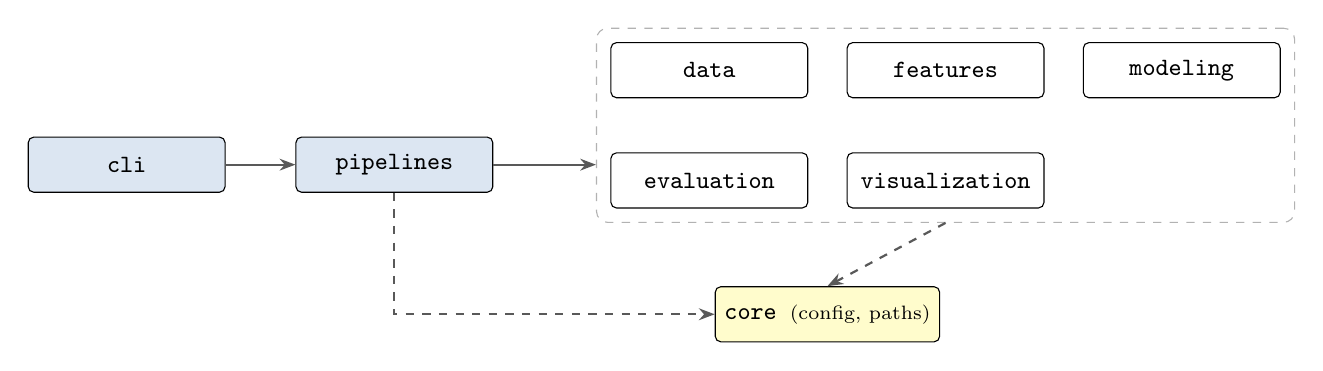
\begin{tikzpicture}[
  box/.style={draw, rounded corners=2pt, minimum height=7mm, minimum width=25mm, font=\small\ttfamily, align=center},
  arr/.style={-{Stealth[length=2mm]}, thick, black!65}
]
\node[box, fill=hdr] (cli) at (0,0) {cli};
\node[box, fill=hdr] (pipe) at (3.4,0) {pipelines};
\foreach \name/\x/\y in {data/7.4/1.2, features/10.4/1.2, modeling/13.4/1.2, evaluation/7.4/-0.2, visualization/10.4/-0.2}
  \node[box, fill=white] (\name) at (\x,\y) {\name};
\node[draw=black!30, dashed, rounded corners, fit=(data)(modeling)(evaluation)(visualization), inner sep=5pt] (leaves) {};
\node[box, fill=yellow!20] (core) at (8.9,-1.9) {core {\rmfamily\scriptsize(config, paths)}};
\draw[arr] (cli) -- (pipe);
\draw[arr] (pipe) -- (leaves.west |- pipe);
\draw[arr, dashed] (leaves.south) -- (core.north);
\draw[arr, dashed] (pipe.south) |- (core.west);
\end{tikzpicture}
\caption{Import direction. \code{cli} only calls \code{pipelines}; \code{pipelines} composes the leaf layers; every layer reads \code{core}. Nothing imports \code{cli} or \code{pipelines}, so each leaf layer is unit-tested in isolation.}
\label{fig:layers}
\end{figure}

The move was a pure \code{git mv} with import fixes, committed separately from any behaviour change. Last week's 42 tests passed unchanged from their new mirrored folders. Pytest now runs with \code{--import-mode=importlib}, because test files in different folders share basenames.

\subsection*{B. AFID Acquisition and Verification}

\code{Codes/scripts/download_afid.sh} fetches the three official archives from the AFID page: \code{NODefect_images.7z} (94\,MB), \code{Defect_images.7z} (74\,MB) and \code{Mask_images.7z} (86\,KB). It extracts them into the git-ignored \code{data/raw/} and skips archives that are already present. The catalog was then checked file by file. Table~\ref{tab:data} gives the composition, and Table~\ref{tab:quirks} lists five quirks of the published archives, each now handled and covered by a test.

\begin{table}[h]
\centering
\caption{AFID defective strips by official defect class and fabric code (verified catalog). Every fabric has 20 defect-free strips, split per fabric into 15 for fitting and 5 held out for calibration.}
\label{tab:data}
\small
\setlength{\tabcolsep}{4.5pt}
\begin{tabular}{@{}lrrrrrrrrr@{}}
\toprule
\textbf{Defect (code)} & \textbf{00} & \textbf{01} & \textbf{02} & \textbf{03} & \textbf{04} & \textbf{05} & \textbf{06} & \textbf{08} & \textbf{All} \\
\midrule
broken end (002) & 3 & 5 & 1 & 0 & 0 & 0 & 0 & 0 & 9 \\
broken yarn (006) & 0 & 0 & 7 & 0 & 1 & 0 & 0 & 0 & 8 \\
broken pick (010) & 0 & 0 & 0 & 10 & 0 & 0 & 0 & 0 & 10 \\
weft curling (016) & 0 & 0 & 0 & 3 & 0 & 0 & 0 & 0 & 3 \\
fuzzy ball (019) & 0 & 1 & 23 & 5 & 6 & 0 & 4 & 0 & 39 \\
cut selvage (022) & 4 & 0 & 0 & 3 & 0 & 0 & 2 & 0 & 9 \\
crease (023) & 0 & 2 & 3 & 0 & 0 & 0 & 0 & 0 & 5 \\
warp ball (025) & 0 & 0 & 0 & 5 & 0 & 0 & 0 & 1 & 6 \\
knot (027) & 0 & 0 & 0 & 0 & 0 & 1 & 0 & 0 & 1 \\
contamination (029) & 0 & 0 & 0 & 0 & 1 & 0 & 0 & 0 & 1 \\
nep (030) & 0 & 3 & 4 & 5 & 2 & 0 & 0 & 0 & 14 \\
weft crack (036) & 0 & 1 & 0 & 0 & 0 & 0 & 0 & 0 & 1 \\
\midrule
\textbf{All} & 7 & 12 & 38 & 31 & 10 & 1 & 6 & 1 & \textbf{106} \\
\bottomrule
\end{tabular}
\end{table}

\begin{table}[h]
\centering
\caption{Quirks found in the published AFID archives and how the pipeline treats them.}
\label{tab:quirks}
\small
\renewcommand{\arraystretch}{1.1}
\begin{tabularx}{\textwidth}{@{}lLL@{}}
\toprule
\textbf{File} & \textbf{Quirk} & \textbf{Handling} \\
\midrule
\code{NODefect_images/2608691-202020u/0018_00_01.png} & 21st defect-free image of fabric 01, with a 2-digit defect field; different content from \code{0018_000_01} & Skipped with a warning (not a valid \code{nnnn_ddd_ff} name) \\
\code{Defect_images/0100_025_08.png} & Fabric code 08 does not exist, and the image has no mask & Skipped with a warning (no reference, no ground truth) \\
\code{0044_019_04}, \code{0097_030_03} & Mask delivered as \code{_mask1} + \code{_mask2} & Parts merged (82 and 81 px) \\
\code{0106_010_03} & Mask file is empty & Evaluated; recall-type metrics NaN \\
\code{0094_027_05.png} & $256\times3796$ instead of 4096 wide & Supported: no fixed width is assumed \\
\bottomrule
\end{tabularx}
\end{table}

The multi-part masks resolve an open question from the mid-semester run. There, \code{0044_019_04} was evaluated with 0 ground-truth pixels and counted as a miss. The old loader looked only for \code{<stem>_mask.png} and never found the two parts, which hold 82 defect pixels together. Of the 106 defective strips, 105 have a mask and a reference fabric and are evaluated.

\subsection*{C. Gabor Filter-Bank Descriptor}

Gabor filters are band-pass filters that are localized in both space and frequency \cite{daugman1985}. A bank of them is a standard texture descriptor \cite{jain1991}. Weaves are periodic, so a filter tuned to the yarn period and orientation responds strongly to intact texture and changes where the period is broken. We use complex filters
\begin{equation}
g_{\lambda,\theta}(x,y)=\exp\!\Big(-\frac{x'^2+\gamma^2y'^2}{2\sigma^2}\Big)\exp\!\Big(i\,\frac{2\pi x'}{\lambda}\Big),\quad
x'=x\cos\theta+y\sin\theta,\; y'=-x\sin\theta+y\cos\theta,
\label{eq:gabor}
\end{equation}
with the even (real) kernel made zero-mean, so that flat regions respond with 0 rather than with their brightness. The envelope width follows from a 1-octave half-response bandwidth $b$ \cite{daugman1985}:
\begin{equation}
\frac{\sigma}{\lambda}=\frac{1}{\pi}\sqrt{\frac{\ln 2}{2}}\;\frac{2^{b}+1}{2^{b}-1}=0.5622\quad(b=1).
\label{eq:bw}
\end{equation}
For each window $W$ and filter, the features are the mean and standard deviation of the magnitude $|I*g_{\lambda,\theta}|$ over $W$, giving $3\times4\times2=24$ values (Table~\ref{tab:gabor}). The responses are computed once per strip, so overlapping windows share the convolutions. Unit tests check the selectivity: vertical stripes with an 8-px period excite $(\lambda{=}8,\theta{=}0^\circ)$ most, horizontal ones $(8,90^\circ)$, and a 16-px period $(16,0^\circ)$.

\begin{table}[h]
\centering
\caption{Gabor bank ($\gamma=0.5$, orientations $0^\circ,45^\circ,90^\circ,135^\circ$). The wavelengths bracket the 4--8\,px AFID yarn period.}
\label{tab:gabor}
\small
\begin{tabular}{@{}rrrl@{}}
\toprule
$\lambda$ (px) & $\sigma$ (px) & kernel size & role \\
\midrule
4 & 2.25 & $15\times15$ & single-yarn scale \\
8 & 4.50 & $29\times29$ & yarn-pair / weave repeat \\
16 & 9.00 & $55\times55$ & coarse structure (creases, curls) \\
\bottomrule
\end{tabular}
\end{table}

The descriptor is now assembled from the blocks named in \code{features.use}: any non-empty subset of \code{glcm} (30-D), \code{lbp} (28-D) and \code{gabor} (24-D). Changing the descriptor is therefore a configuration change, not a code change.

\subsection*{D. Feature Cache and Parallel Extraction}

Profiling last week showed that feature extraction dominates run time, while fitting and scoring take milliseconds. Each strip's window features are now computed \emph{once} for every block (GLCM, LBP, Gabor) and every window geometry. They are stored as compressed \code{.npz} files under \code{data/processed/} and reused by every run that only changes modelling, scoring or threshold settings. The cache key hashes only the settings that change the numbers (pre-processing, GLCM, LBP and Gabor parameters). Each file is keyed by the image path, size and modification time, so an edited image is recomputed automatically. Files are written atomically (temporary file, then rename), so an interrupted run cannot leave a corrupt entry. LBP codes and Gabor responses are now computed once per strip and then pooled per window. Previously they were recomputed for every overlapping patch, which also means border codes now see their true neighbours. Extraction runs in a standard-library process pool (\code{--workers}).

\begin{table}[h]
\centering
\caption{Wall-clock times on all 246 AFID strips (8 worker processes, laptop CPU).}
\label{tab:time}
\small
\begin{tabular}{@{}lr@{}}
\toprule
\textbf{Run} & \textbf{Time} \\
\midrule
Cold cache, $256\times256$ windows, all three blocks & 60.5\,s \\
Cold cache, $256\times256$ and $64\times64$ windows (default) & 163.1\,s \\
Warm cache, full default benchmark incl.\ figures & 10.4\,s \\
Warm cache, 15-variant ablation (Section~I) & 57.4\,s \\
\bottomrule
\end{tabular}
\end{table}

Without the cache, the 15-variant ablation would repeat up to 163\,s of extraction per variant (up to about 40 minutes). With the cache it takes under a minute.

\subsection*{E. Nested $64\times64$ Refinement}

A $256\times256$ window gives stable texture statistics, but when it is flagged all 65{,}536 of its pixels enter the mask, even for a thread a few pixels wide. That capped pixel IoU near zero in every earlier report. Refinement keeps the coarse decision as a region of interest and re-decides inside it at a finer scale. Let $\mathcal{F}$ be the flagged coarse windows of a strip and
\begin{equation}
R=\bigcup_{w\in\mathcal{F}} w,\qquad
\hat{M}=\mathrm{morph}\Big(\bigcup\big\{\,v : v\subseteq R,\; d^{(64)}_f(\mathbf{x}_v)\ge\tau^{(64)}_f\,\big\}\Big),
\label{eq:refine}
\end{equation}
where $v$ ranges over the $64\times64$ windows (stride 32) of the strip, and $d^{(64)}_f$ is the Mahalanobis distance to a \emph{second} reference of fabric $f$. That reference is fitted on $64\times64$ windows of the same 15 fit images. Its threshold $\tau^{(64)}_f$ is calibrated on the same 5 held-out images with the same $\mu+k\sigma$ rule ($k=2.5$). The containment test $v\subseteq R$ uses a summed-area table \cite{crow1984}, one $O(1)$ lookup per window. ``morph'' is the existing $5\times5$ opening and closing with removal of components under 50\,px. Patch-level metrics still use the coarse decision; refinement changes only the pixel mask.

\subsection*{F. One-Class Baselines}

To test whether a simple Gaussian model of normal texture is adequate, we added two learned one-class detectors \cite{scholkopf2001,liu2008}. They run on the same descriptors, the same fit and calibration images and the same threshold rule. Features are standardised on the fit set. The anomaly score is the negated decision function, so that higher means more anomalous, and $\tau=\mu+k\sigma$ on the held-out images. The One-Class SVM uses an RBF kernel with $\nu=0.1$ and \code{gamma="scale"}. The Isolation Forest uses 200 trees and is seeded. Only the scoring function differs from the Mahalanobis reference.

\subsection*{G. Adaptive (Per-Fabric) vs.\ Fixed (Global) Reference}

The project's central design choice is \emph{adaptivity}: a separate texture model and threshold for each fabric. \code{model.reference = "global"} implements the fixed alternative. It pools the fit images of all seven fabrics into one model, pools all calibration images into one $\tau$, and applies both to every strip. The images used are identical in both settings; only the pooling differs.

\subsection*{H. Strip-Normalised Mahalanobis Scoring}

The full benchmark revealed a capture shift between defect-free and defective strips (Section ``Discussion'', Table~\ref{tab:shift}). As a remedy we added \code{strip_mahalanobis}: the Mahalanobis distances of one strip, converted to one-sided robust $z$-scores within that strip,
\begin{equation}
s_i=\max\!\Big(0,\ \frac{d_f(\mathbf{x}_i)-\operatorname{med}_j d_f(\mathbf{x}_j)}{\operatorname{MAD}_j d_f(\mathbf{x}_j)+10^{-4}}\Big),\qquad \text{flag if } s_i\ge k,
\label{eq:strip}
\end{equation}
which removes any strip-wide offset while keeping the fabric model's notion of what is normal \cite{rousseeuw1993}.

\subsection*{I. Ablation Protocol and Pooled Metrics}

\code{python -m fabric_defect ablate --grid Codes/configs/experiments/ablation.toml} runs 15 named variants. Each variant changes \emph{one} factor relative to the default (one factor at a time), and all share the same seed. They therefore use the same image-level split, the same 105 test strips and the same cached features, and differences come only from the named factor. The summary reports per-image means (NaN-skipping, as introduced in Week~5) and \emph{pooled} metrics, which sum TP/FP/FN over all strips before forming ratios:
\begin{equation}
\mathrm{IoU}_{\text{pooled}}=\frac{\sum_i TP_i}{\sum_i (TP_i+FP_i+FN_i)},\qquad
F1_{\text{pooled}}=\frac{2\sum_i TP_i}{\sum_i (2\,TP_i+FP_i+FN_i)}.
\label{eq:pooled}
\end{equation}
Per-image means give a 15-px warp ball the same weight as a full-width crease. Pooled metrics give every pixel (or patch) the same weight. Both views are reported because they can disagree.

%=====================================================================
\section*{Quantitative Results and Analysis}

All numbers in this section are on \textbf{real AFID data}: the 105 defective strips that have a mask, with references fitted on 15 and calibrated on 5 defect-free strips per fabric (seed 0). The raw per-strip results are in \code{Results/final/} and \code{Results/ablation/}, each with its \code{run_config.json}.

\subsection*{Headline Result}

\begin{table}[h]
\centering
\caption{Default configuration vs.\ the Week-5 setting on all 105 strips (per-image means unless marked pooled).}
\label{tab:headline}
\small
\begin{tabularx}{\textwidth}{@{}>{\raggedright\arraybackslash}p{0.33\textwidth}CCCCC@{}}
\toprule
\textbf{Setting} & \textbf{Patch F1} & \textbf{Pooled patch F1} & \textbf{Pixel IoU} & \textbf{Pooled pixel IoU} & \textbf{Pixel recall} \\
\midrule
Week-5 setting: hybrid, GLCM+LBP, no refinement & 13.97 & 14.78 & 0.30 & 0.33 & 32.73 \\
\textbf{Default}: Mahalanobis, GLCM+LBP, $64\times64$ refinement & \textbf{18.14} & \textbf{22.74} & \textbf{1.36} & \textbf{1.12} & \textbf{48.39} \\
\bottomrule
\end{tabularx}
\end{table}

\subsection*{Ablation}

\begin{table}[h]
\centering
\caption{One-factor-at-a-time ablation around the default (all values in \%, AFID, $n=105$). Bold: default. Prec./Rec./Spec.\ are per-image patch metrics.}
\label{tab:ablation}
\small
\setlength{\tabcolsep}{2.6pt}
\begin{tabularx}{\textwidth}{@{}lRRRRRRRR@{}}
\toprule
\textbf{Variant} & \textbf{Prec.} & \textbf{Rec.} & \textbf{F1} & \textbf{F1 pool.} & \textbf{Spec.} & \textbf{IoU} & \textbf{IoU pool.} & \textbf{Pix.\ rec.} \\
\midrule
\textbf{default} & \textbf{18.67} & \textbf{63.19} & \textbf{18.14} & \textbf{22.74} & \textbf{55.29} & \textbf{1.36} & \textbf{1.12} & \textbf{48.39} \\
\addlinespace
\multicolumn{9}{@{}l}{\emph{Descriptor}} \\
GLCM only & 19.25 & 62.97 & 18.74 & 22.63 & 55.32 & 1.36 & 1.12 & 48.17 \\
LBP only & 11.81 & 52.66 & 11.73 & 21.58 & 56.46 & 1.09 & 1.10 & 38.75 \\
Gabor only & 13.11 & 70.65 & 15.49 & 22.79 & 42.44 & 0.90 & 1.05 & 56.47 \\
GLCM+LBP+Gabor & 15.25 & 72.47 & 16.95 & 22.85 & 42.34 & 1.05 & 1.01 & 56.79 \\
\addlinespace
\multicolumn{9}{@{}l}{\emph{Scoring}} \\
strip Mahalanobis & 16.72 & 15.13 & 9.24 & 13.33 & 92.13 & 0.46 & 0.86 & 9.33 \\
hybrid (Week 5) & 13.44 & 32.41 & 13.97 & 14.78 & 75.91 & 0.72 & 0.67 & 27.18 \\
relative & 13.41 & 39.10 & 14.57 & 16.57 & 72.93 & 0.88 & 0.90 & 30.41 \\
\addlinespace
\multicolumn{9}{@{}l}{\emph{Learned baselines}} \\
One-Class SVM & 17.78 & 55.55 & 16.47 & 23.41 & 58.80 & 1.30 & 1.11 & 43.65 \\
Isolation Forest & 20.84 & 48.40 & 13.96 & 17.96 & 64.36 & 0.85 & 0.89 & 39.39 \\
\addlinespace
\multicolumn{9}{@{}l}{\emph{Reference / threshold}} \\
global (fixed) reference & 11.46 & 26.85 & 5.78 & 12.03 & 75.51 & 0.07 & 0.10 & 22.82 \\
$k=2.0$ & 18.25 & 69.77 & 19.38 & 23.36 & 52.09 & 1.38 & 1.12 & 50.74 \\
$k=3.0$ & 19.69 & 59.07 & 18.40 & 22.14 & 57.47 & 1.34 & 1.11 & 46.89 \\
\addlinespace
\multicolumn{9}{@{}l}{\emph{Localization}} \\
refinement off & 18.67 & 63.19 & 18.14 & 22.74 & 55.29 & 0.70 & 0.92 & 53.89 \\
Week-5 setting (all three changes) & 13.44 & 32.41 & 13.97 & 14.78 & 75.91 & 0.30 & 0.33 & 32.73 \\
\bottomrule
\end{tabularx}
\end{table}

\paragraph{How the default was chosen.} A first pass around the Week-5 default (hybrid scoring) favoured all three descriptor blocks and Mahalanobis scoring. Re-centring on Mahalanobis + refinement showed that Gabor's gain belonged to the hybrid scorer. Under Mahalanobis, adding Gabor raises patch recall (63.2 $\rightarrow$ 72.5\,\%), but it lowers precision and specificity (55.3 $\rightarrow$ 42.3\,\%), patch F1 (18.1 $\rightarrow$ 17.0\,\%) and IoU (1.36 $\rightarrow$ 1.05\,\%). The default is therefore GLCM+LBP, with Gabor available as an option. GLCM alone is within noise of GLCM+LBP. We keep both, since the patch-level differences are a few strips. $k=2.0$ scores marginally higher, but it is \emph{not} adopted: picking $k$ on the test strips would bias the result. $k$ stays at the a-priori 2.5.

\subsection*{Per-Fabric and Per-Defect Results (Default)}

\begin{table}[h]
\centering
\caption{Default configuration per fabric (\%, per-image means), with the capture-shift statistics of Table~\ref{tab:shift} for comparison.}
\label{tab:fabric}
\small
\begin{tabularx}{\textwidth}{@{}lrRRRRRR@{}}
\toprule
\textbf{Fabric} & $n$ & \textbf{Patch prec.} & \textbf{Patch rec.} & \textbf{Patch F1} & \textbf{Pixel IoU} & \textbf{Pixel rec.} & \textbf{FP rate on normal windows} \\
\midrule
fabric\_00 & 7 & 6.90 & 57.14 & 9.07 & 0.06 & 57.14 & 57.33 \\
fabric\_01 & 12 & 14.73 & 100.00 & 20.89 & 1.93 & 89.15 & 93.63 \\
fabric\_02 & 38 & 4.09 & 75.00 & 7.42 & 0.09 & 55.26 & 53.83 \\
fabric\_03 & 31 & \textbf{39.95} & 63.15 & \textbf{34.30} & \textbf{3.73} & 39.08 & 31.94 \\
fabric\_04 & 10 & 0.00 & 0.00 & 0.00 & 0.00 & 0.00 & 1.72 \\
fabric\_05 & 1 & 6.90 & 100.00 & 12.90 & 0.03 & 100.00 & 100.00 \\
fabric\_06 & 6 & 25.00 & 30.00 & 25.00 & 0.07 & 31.67 & 9.09 \\
\bottomrule
\end{tabularx}
\end{table}

\begin{table}[h]
\centering
\caption{Default configuration per official defect class (\%, per-image means). ``--'' = undefined: no window of any of these strips holds more than 25 mask pixels.}
\label{tab:defect}
\small
\begin{tabularx}{\textwidth}{@{}lrRRRRR@{}}
\toprule
\textbf{Defect} & $n$ & \textbf{Patch prec.} & \textbf{Patch rec.} & \textbf{Patch F1} & \textbf{Pixel IoU} & \textbf{Pixel rec.} \\
\midrule
broken pick (010) & 10 & 76.00 & 57.28 & 50.65 & 10.91 & 47.76 \\
weft crack (036) & 1 & 93.55 & 100.00 & 96.67 & 22.39 & 98.83 \\
cut selvage (022) & 9 & 51.14 & 44.44 & 36.83 & 0.21 & 43.34 \\
weft curling (016) & 3 & 15.48 & 50.00 & 23.61 & 1.57 & 47.53 \\
crease (023) & 5 & 8.57 & 60.00 & 14.54 & 0.49 & 80.00 \\
broken end (002) & 9 & 6.53 & 88.89 & 12.14 & 0.11 & 85.66 \\
knot (027) & 1 & 6.90 & 100.00 & 12.90 & 0.03 & 100.00 \\
broken yarn (006) & 8 & 6.91 & 87.50 & 11.30 & 0.12 & 87.50 \\
fuzzy ball (019) & 39 & 7.70 & 50.00 & 9.42 & 0.01 & 25.64 \\
nep (030) & 14 & 4.73 & 69.23 & 8.79 & 0.02 & 64.29 \\
warp ball (025) & 5 & 0.00 & -- & 0.00 & 0.02 & 20.00 \\
contamination (029) & 1 & 0.00 & 0.00 & 0.00 & 0.00 & 0.00 \\
\bottomrule
\end{tabularx}
\end{table}

\subsection*{The AFID Capture Shift}

\begin{table}[h]
\centering
\caption{Default-config Mahalanobis distance ($256\times256$) per fabric: held-out \emph{defect-free} calibration strips vs.\ the \emph{normal} windows (no defect pixels above the 25-px rule) of the defective test strips.}
\label{tab:shift}
\small
\begin{tabularx}{\textwidth}{@{}lrRRRRR@{}}
\toprule
\textbf{Fabric} & $\tau_f$ & \textbf{Calib.\ median} & \textbf{Calib.\ FP rate (\%)} & \textbf{Test-normal windows} & \textbf{Test-normal median} & \textbf{Test-normal FP rate (\%)} \\
\midrule
fabric\_00 & 4.03 & 2.44 & 0.93 & 150 & 6.96 & 57.33 \\
fabric\_01 & 4.44 & 2.50 & 2.90 & 314 & 12.95 & 93.63 \\
fabric\_02 & 4.58 & 2.45 & 1.38 & 1{,}098 & 12.82 & 53.83 \\
fabric\_03 & 4.42 & 2.72 & 1.74 & 551 & 3.54 & 31.94 \\
fabric\_04 & 4.55 & 2.35 & 1.29 & 291 & 2.04 & 1.72 \\
fabric\_05 & 4.20 & 2.29 & 2.76 & 27 & 23.09 & 100.00 \\
fabric\_06 & 3.71 & 2.25 & 3.23 & 176 & 2.45 & 9.09 \\
\bottomrule
\end{tabularx}
\end{table}

\begin{figure}[h]
\centering
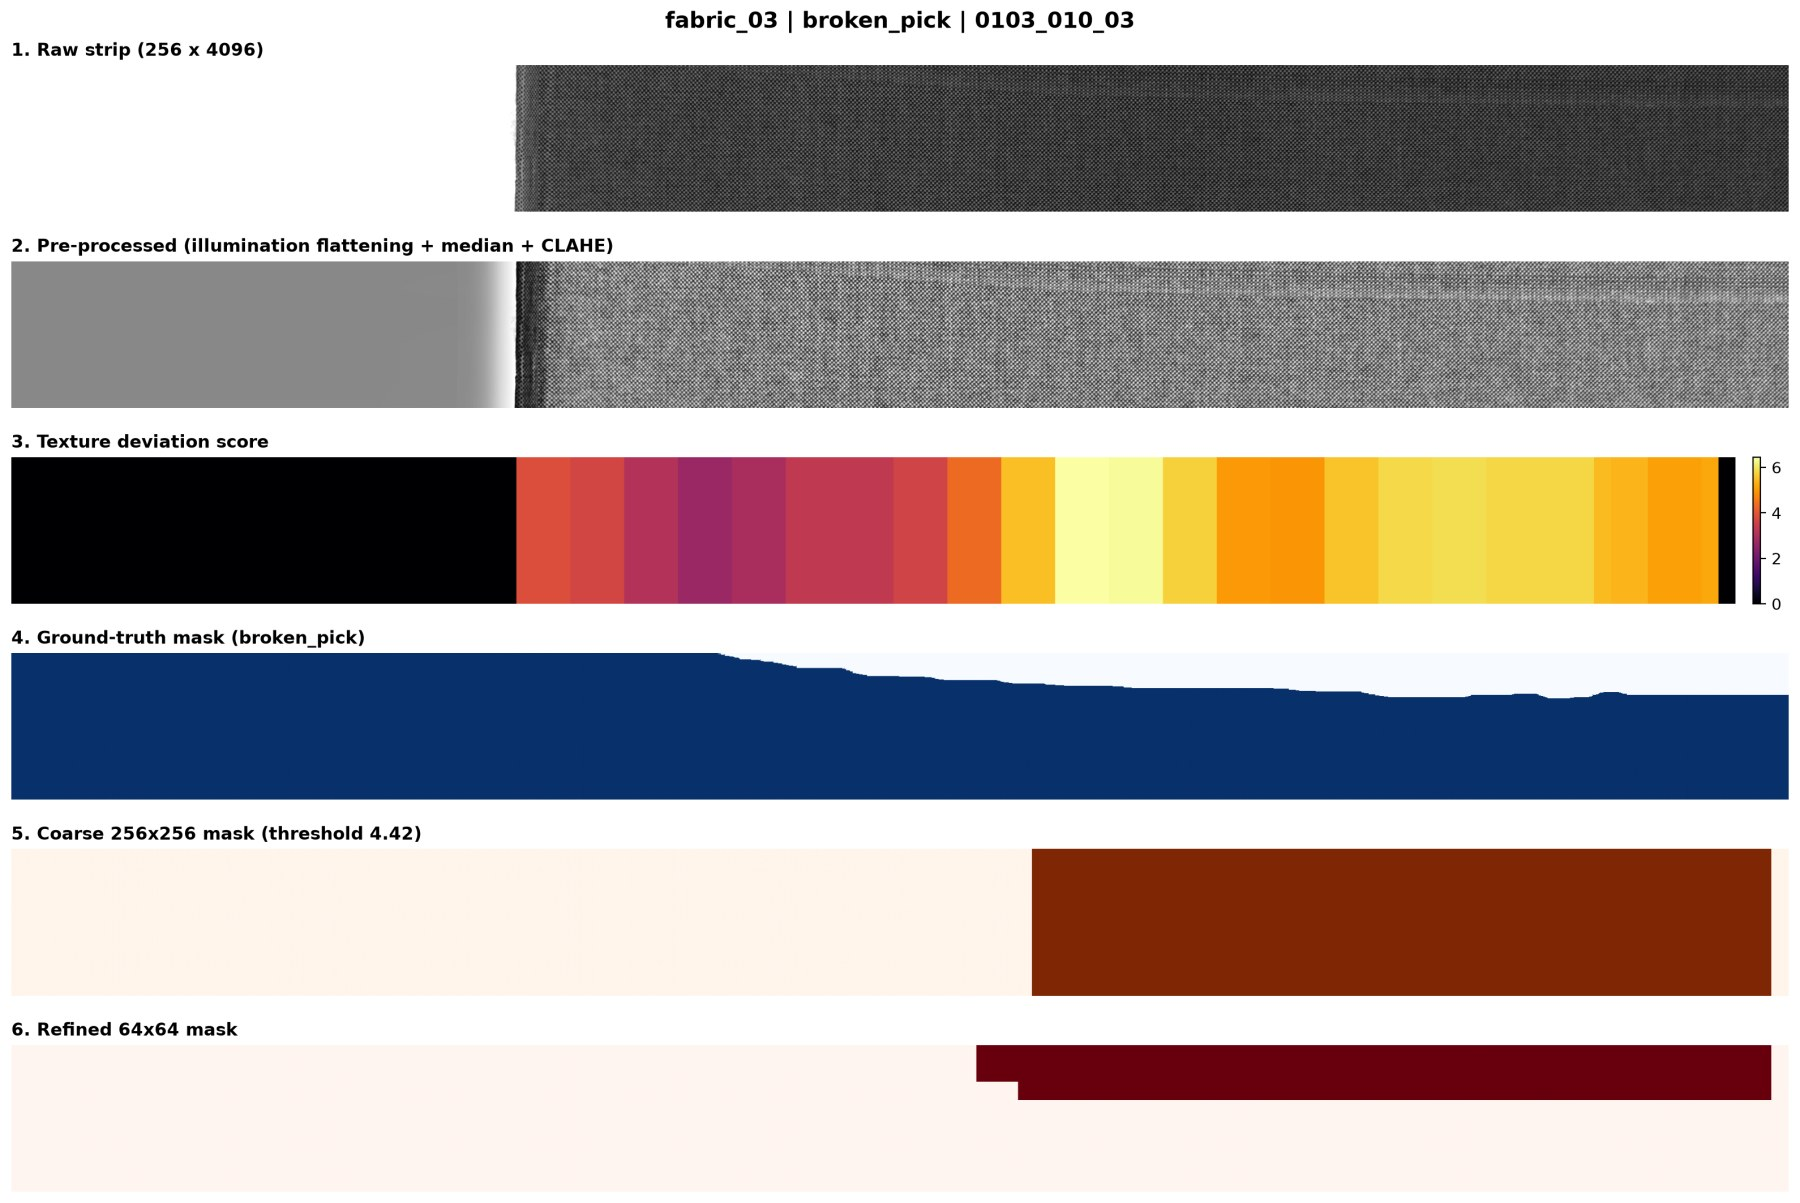
\includegraphics[width=0.95\textwidth]{figures/afid_0103_010_03_best.jpg}
\caption{Success case, AFID \code{0103_010_03} (broken pick, fabric\_03): pixel IoU 63.3\,\%, pixel recall 85.5\,\%. The $256\times256$ decision (panel~5) flags the right half of the strip. The $64\times64$ refinement (panel~6) reduces it to the band along the top rows where the pick is missing (white region in panel~4).}
\label{fig:best}
\end{figure}

\begin{figure}[h]
\centering
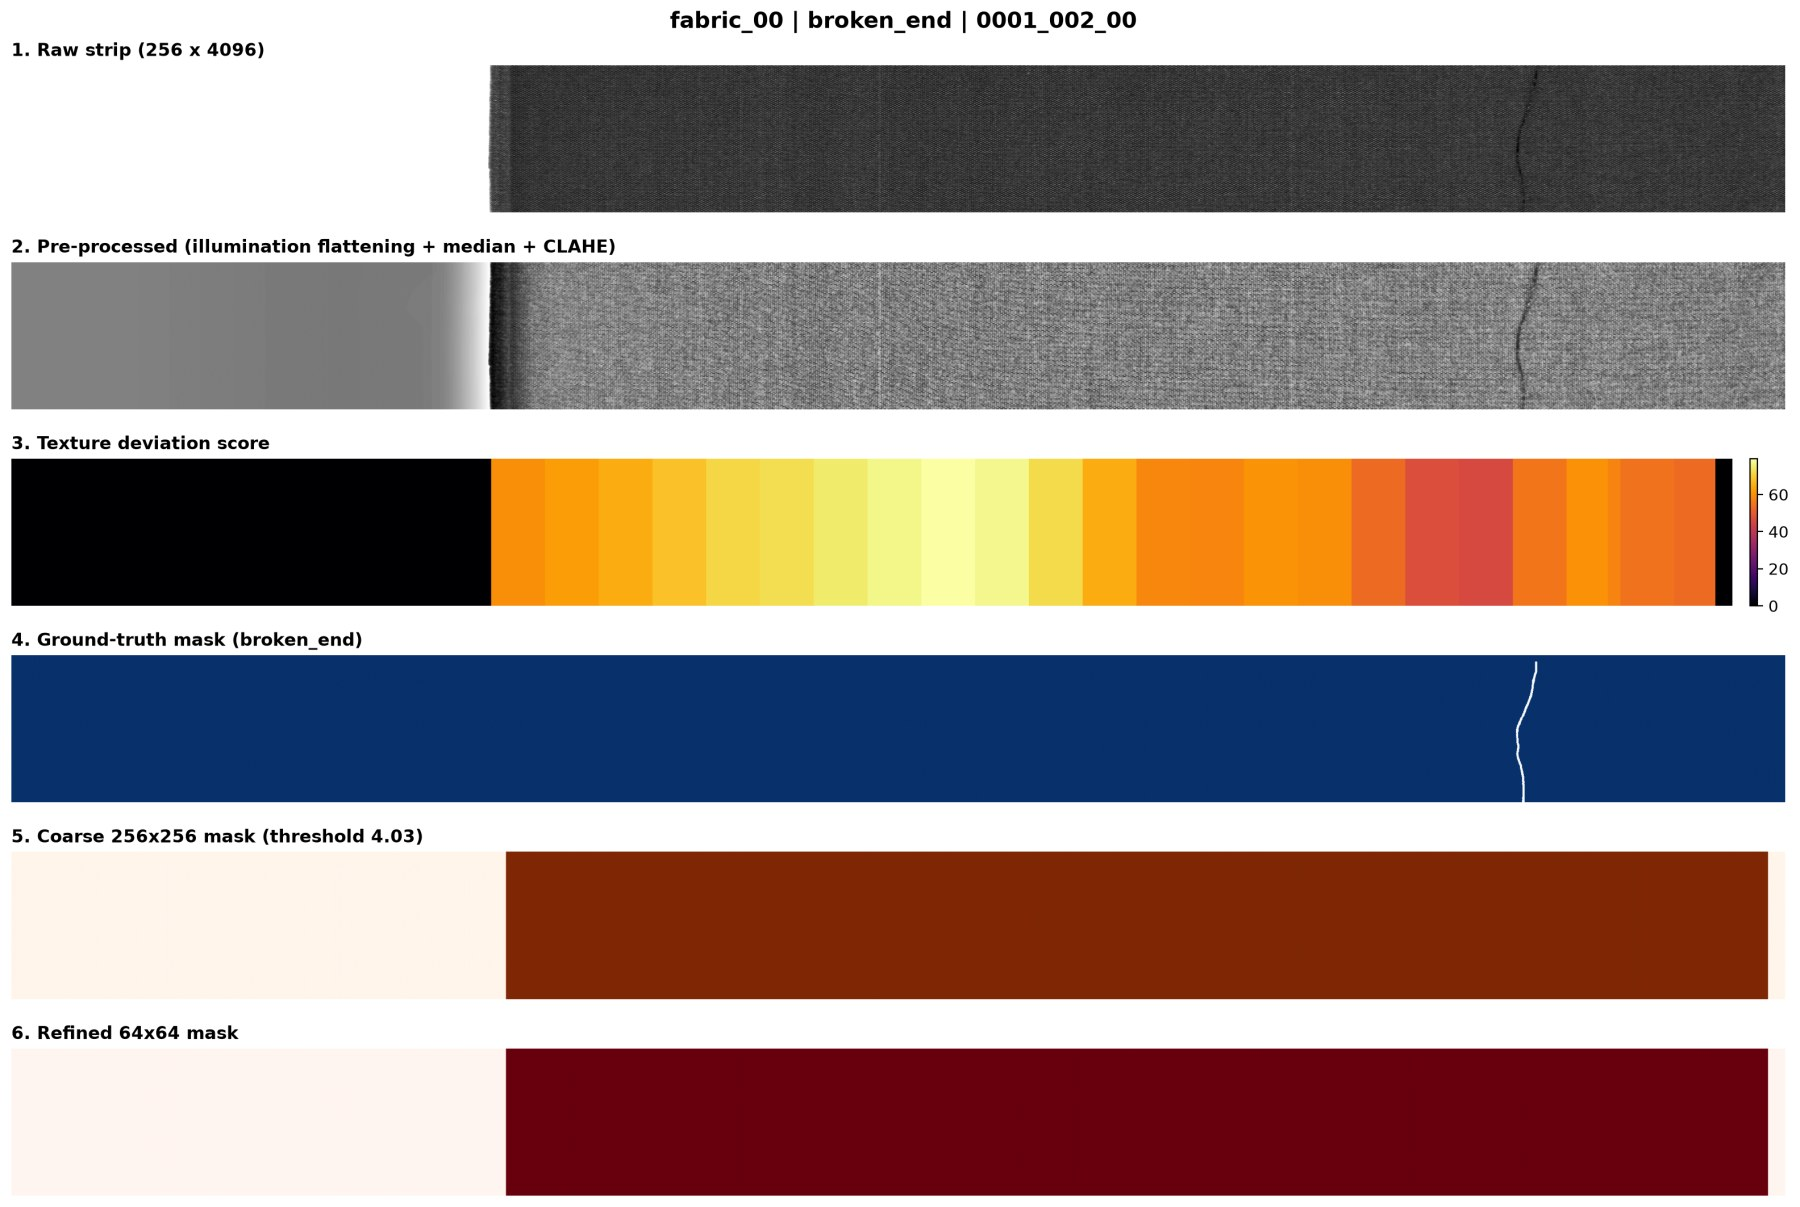
\includegraphics[width=0.95\textwidth]{figures/afid_0001_002_00.jpg}
\caption{Failure case caused by the capture shift, AFID \code{0001_002_00} (broken end, fabric\_00). Every window of the strip scores 40--70 against $\tau=4.03$ (panel~3), so both the coarse and the refined mask cover the whole fabric. The defect (panel~4) is found, but precision is near zero.}
\label{fig:fail}
\end{figure}

\begin{figure}[h]
\centering
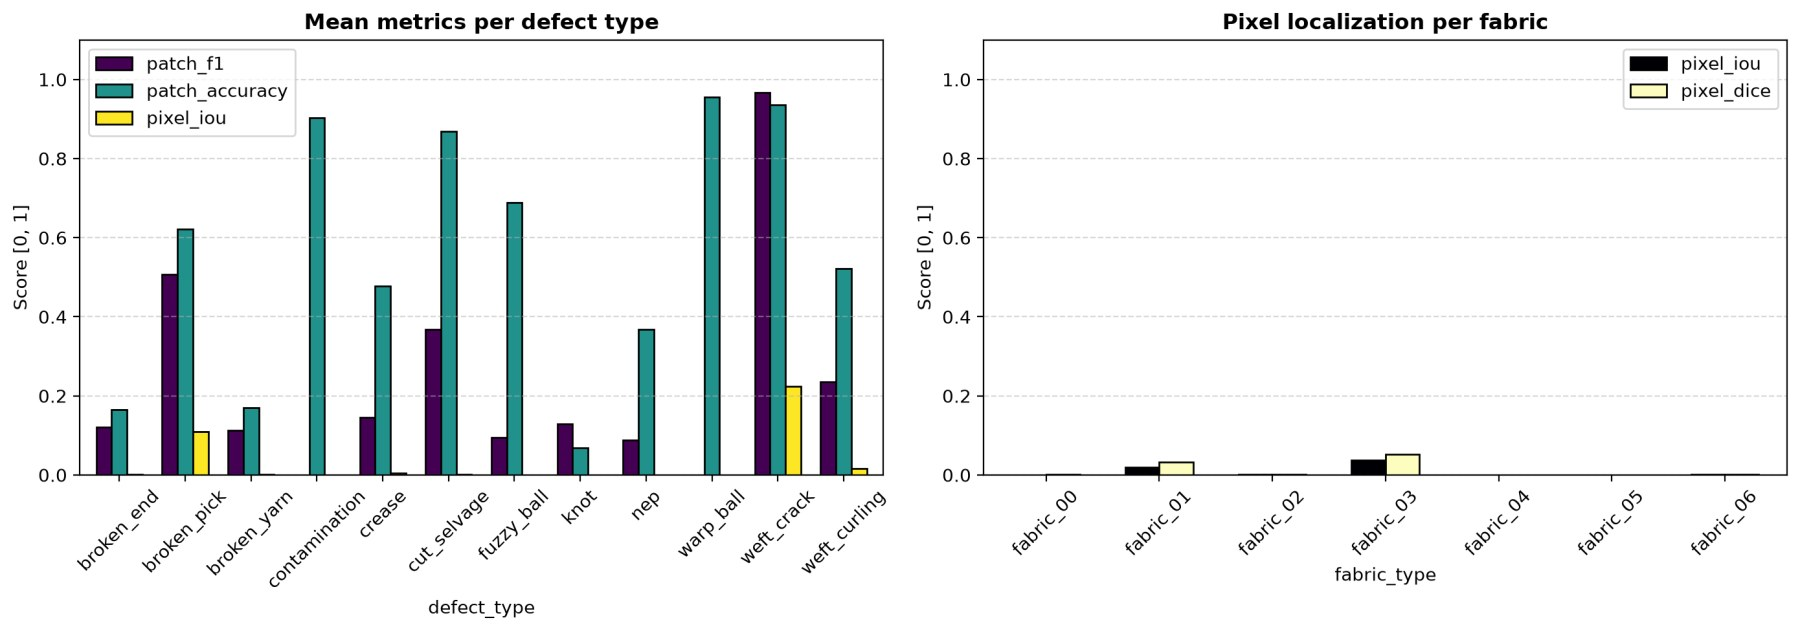
\includegraphics[width=0.92\textwidth]{figures/charts.jpg}
\caption{Mean metrics per official defect class and per fabric for the default configuration (from \code{Results/final/figures/}).}
\label{fig:charts}
\end{figure}

%=====================================================================
\section*{Discussion of Findings}
\begin{enumerate}
  \item \textbf{Adaptivity is justified by data.} Replacing the per-fabric references and thresholds with one global model is the largest single degradation in the ablation. Patch F1 falls from 18.14 to 5.78\,\%, pixel IoU from 1.36 to 0.07\,\% and pixel recall from 48.4 to 22.8\,\%. The seven weaves occupy different regions of descriptor space, so a single covariance spans all of them, and a pooled $\tau$ is too loose for some fabrics and too tight for others.
  \item \textbf{The capture shift sets the false-positive floor.} On held-out \emph{defect-free} strips the thresholds behave exactly as calibrated (0.9--3.2\,\% false positives, Table~\ref{tab:shift}). On defect-free \emph{windows of defective strips} the rate is 32--100\,\% for fabrics 00, 01, 02, 03 and 05, whose median distances are 1.3--10$\times$ the calibration median. Only fabrics 04 and 06 transfer (1.7\,\% and 9.1\,\%). This matches the per-fabric precision in Table~\ref{tab:fabric}, and Figure~\ref{fig:fail} shows the effect. AFID's defect-free and defective images appear to come from different acquisitions (rolls, tension or lighting), a dataset shift in the sense of \cite{quinonero2009}. It explains why the Week-5 strip-relative scores were introduced. It is also why every scorer, learned or not, stays below about 20\,\% patch precision: the scorers differ in how they trade recall for specificity, not in whether they see the shift.
  \item \textbf{Strip normalisation buys specificity, not accuracy.} \code{strip_mahalanobis} removes the offset (specificity 92.1\,\%) but also suppresses defects that span many windows, so recall drops to 15\,\%. It is a useful high-precision operating point, not a better default. A correct fix needs reference data from the same acquisition as the test strips (see Plan).
  \item \textbf{Refinement doubles localization quality.} Refinement leaves patch decisions unchanged by design, and it raises mean pixel IoU from 0.70 to 1.36\,\% and pooled IoU from 0.92 to 1.12\,\%. In return, pixel recall drops from 53.9 to 48.4\,\% where a fine window falls just below $\tau^{(64)}$. Where the coarse decision is right, the effect is large (Figure~\ref{fig:best}: 63\,\% IoU). Where the capture shift has flagged everything, refinement cannot help, because the fine model shifts too.
  \item \textbf{GLCM carries the descriptor.} GLCM alone matches GLCM+LBP. LBP alone is weakest (F1 11.7\,\%), as its histograms change little for thin defects inside a $256\times256$ window. Gabor alone reaches the highest recall of any descriptor (70.7\,\%), but at the lowest specificity. The tuned band-pass responses react to the shift as well as to defects.
  \item \textbf{The Gaussian model is competitive with learned one-class methods.} The One-Class SVM edges the default on pooled patch F1 (23.4 vs.\ 22.7\,\%). It is below on mean F1 (16.5 vs.\ 18.1\,\%), IoU (1.30 vs.\ 1.36\,\%) and recall. The Isolation Forest is clearly weaker (F1 14.0\,\%). With 15 fit images per fabric, a regularised mean and covariance are as good a description of normal texture as these learned boundaries, and far cheaper.
  \item \textbf{Defect classes split by geometry.} Weft-direction defects that span the strip width are found and localised best: broken pick (F1 50.7\,\%, IoU 10.9\,\%), weft crack and cut selvage. Small, compact defects are the hardest: fuzzy ball ($n=39$, IoU 0.01\,\%), nep and warp ball. All five warp-ball masks have only 11--24 pixels, below the 25-pixel patch-label rule, so their patch recall is undefined rather than zero. Fabric\_04 is the extreme case. It has almost no capture shift, but its defects are all small (6 fuzzy balls, 2 neps, 1 broken yarn, 1 contamination) and none is detected.
  \item \textbf{Absolute levels remain low.} Even the best configuration localises about 1\,\% of defect pixels correctly by IoU. The improvements are real and reproducible (pixel IoU $\times4.5$, recall $+15.7$ points over the Week-5 setting), but the system is far from usable inspection accuracy. The capture shift and small defects are the two bottlenecks, and both are now quantified.
\end{enumerate}

%=====================================================================
\section*{Testing and Continuous Integration}

The suite grew from 42 to 72 tests (about 2 minutes, including synthetic end-to-end runs of both subcommands), mirrored into \code{tests/\{data, features, modeling, evaluation, pipelines, cli\}/}. New tests cover the following.
\begin{itemize}
  \item \textbf{Data.} The malformed AFID filename is skipped.
  \item \textbf{Gabor.} One-octave $\sigma$ (Eq.~\ref{eq:bw}); orientation and wavelength selectivity on synthetic stripes; zero response on flat images; block selection in the descriptor.
  \item \textbf{Cache.} ROI-relative coordinates; round trip through the cache with 1 vs.\ 2 workers (bit-identical); separate cache entries when feature settings change; reuse when only modelling settings change; per-scale reuse.
  \item \textbf{Modelling.} Refinement region, containment by summed-area table (vs.\ brute force) and the refined mask; OC-SVM and Isolation Forest rank outliers above normal data and are seeded; strip normalisation removes a global offset; the global reference shares one model across fabrics.
  \item \textbf{Evaluation.} Pooled vs.\ mean pixel IoU on a two-image example.
  \item \textbf{Pipelines and CLI.} Grid parsing, duplicate or unknown keys rejected, \code{ablate} end-to-end through the CLI, exit code~2 for a bad grid.
\end{itemize}
GitHub Actions runs the suite on Python 3.11 and 3.13 on every push and pull request.

\section*{Commit History}

\begin{longtable}{@{}lp{0.80\textwidth}@{}}
\caption{Commits of the week on \code{feat/week-6}, oldest first (single-purpose, one-line messages).}\label{tab:commits}\\
\toprule
\textbf{Hash} & \textbf{Message} \\
\midrule
\endfirsthead
\toprule
\textbf{Hash} & \textbf{Message} \\
\midrule
\endhead
\code{bf91e67} & refactor: move package to src layout with layered subpackages \\
\code{242935c} & chore: add AFID download script and skip malformed AFID filenames \\
\code{42fc4d5} & feat: add Gabor filter-bank descriptor and configurable feature blocks \\
\code{c994611} & feat: cache window features per image and extract them in parallel \\
\code{5c97f1f} & feat: refine flagged patches at 64x64 against a fine-scale reference \\
\code{6e32ebf} & feat: add One-Class SVM and Isolation Forest baselines \\
\code{ef323e8} & feat: add ablation runner and a global reference for fixed-vs-adaptive comparison \\
\code{a86fd92} & feat: report pooled patch and pixel metrics alongside per-image means \\
\code{5fe1048} & feat: add strip-normalised Mahalanobis scoring for the AFID capture shift \\
\code{6dd5f82} & feat: default to Mahalanobis on GLCM+LBP+Gabor with 64x64 refinement \\
\code{5d2fcd6} & fix: keep GLCM+LBP as the default descriptor after the Mahalanobis ablation \\
\code{3b8b940} & chore: publish full AFID benchmark and ablation results and archive legacy outputs \\
\code{7f24fdc} & docs: update README for src layout, AFID download and Week 6 results \\
\bottomrule
\end{longtable}

\noindent The two default-changing commits are kept as they happened. Commit \code{6dd5f82} adopted the first-pass winner; \code{5d2fcd6} reverted the descriptor part after the re-centred ablation (Section ``Ablation'').

%=====================================================================
\section*{Literature Review}

\begin{center}
\small
\renewcommand{\arraystretch}{1.15}
\begin{longtable}{@{}p{0.25\textwidth}p{0.35\textwidth}p{0.33\textwidth}@{}}
\toprule
\rowcolor{hdr}\textbf{Topic / Paper} & \textbf{Key Takeaway} & \textbf{Relevance to the Project} \\
\midrule
\endhead
src layout vs.\ flat layout (PyPA) \cite{pypa} & Importable code under \code{src/} must be installed before it can be imported; tests then run against the installed package and stray files cannot shadow it. & Basis of the new \code{Codes/src/} layout and the editable install used in development and CI. \\
Cookiecutter Data Science \cite{ccds} & A conventional project tree: raw and processed data outside the code; dataset, features, modelling and plotting as separate modules. & Basis of the subpackage split (Table~\ref{tab:map}) and of \code{data/processed} as the feature-cache location. \\
Unsupervised texture segmentation using Gabor filters \cite{jain1991} & A bank of Gabor filters at several frequencies and orientations, with local energy statistics, separates textures. & The 24-D Gabor block (Eq.~\ref{eq:gabor}, Table~\ref{tab:gabor}). \\
Uncertainty relation for 2-D visual filters \cite{daugman1985} & Gabor functions achieve the joint space--frequency resolution limit; bandwidth sets $\sigma/\lambda$. & The one-octave $\sigma=0.5622\lambda$ rule (Eq.~\ref{eq:bw}). \\
Estimating the support of a high-dimensional distribution \cite{scholkopf2001} & One-Class SVM: a kernel boundary around the training data with outlier fraction bounded by $\nu$. & Learned baseline; nearly matches but does not beat the Mahalanobis reference. \\
Isolation Forest \cite{liu2008} & Anomalies are isolated by fewer random splits; linear-time, no density estimate. & Second baseline; weaker than both other scorers on AFID. \\
Summed-area tables \cite{crow1984} & Any rectangle sum in $O(1)$ after one cumulative pass. & Fast ``fine window inside coarse region'' test in refinement (Eq.~\ref{eq:refine}). \\
Dataset Shift in Machine Learning \cite{quinonero2009} & Training and test distributions can differ; models calibrated on one can fail on the other. & Frames the AFID capture shift (Table~\ref{tab:shift}) as the main open problem. \\
AFID \cite{silvestre2019} & Public benchmark: 7 fabrics, 12 defect classes, pixel masks. & Dataset; checked and its quirks documented (Tables~\ref{tab:data}, \ref{tab:quirks}). \\
GLCM \cite{haralick1973}; LBP \cite{ojala2002} & Co-occurrence statistics; rotation-invariant uniform local binary patterns. & The default GLCM+LBP descriptor; GLCM shown to carry most of the signal. \\
\bottomrule
\end{longtable}
\end{center}

\section*{Challenges Faced}
\begin{itemize}
  \item \textbf{Dataset quirks.} The archives contain an extra, misnamed defect-free image, a defective image of a non-existent fabric without a mask, two split masks, one empty mask and one shorter strip (Table~\ref{tab:quirks}). Each now has explicit handling and a test, rather than silently changing the counts.
  \item \textbf{Capture shift.} The largest effect in the results is a property of the data, not of any method. It took a dedicated measurement (Table~\ref{tab:shift}) to separate it from descriptor and scorer choices, and it limits what any defect-free-trained detector can reach on AFID.
  \item \textbf{Avoiding test-set tuning.} With 105 strips and no separate validation set of defective images, every default choice risks fitting the test set. We fixed $k=2.5$ a priori, chose defaults only between methods (not fine parameter values), and report the full ablation so the reader can see every alternative.
  \item \textbf{Run time.} The first full runs took minutes per configuration. The per-image cache made iterating over 15+ variants practical (Table~\ref{tab:time}).
\end{itemize}

\section*{Plan for Next Week (Week 7)}
\begin{itemize}
  \item \textbf{Image-level detection and confidence score.} Add the 35 held-out defect-free strips to the test set to measure image-level false alarms, which the defective-only protocol cannot measure. Derive a per-image confidence from the strip's maximum normalised distance.
  \item \textbf{Address the capture shift.} Calibrate on defect-free regions of defective strips using a strip-level split that never shares a strip between calibration and testing. Also evaluate a per-strip offset correction applied only to the background distribution, which keeps the recall that full strip normalisation loses.
  \item \textbf{Small defects.} Evaluate a $32\times32$ refinement level and a lower patch-label rule for fuzzy balls, neps and warp balls (11--24\,px masks).
  \item \textbf{End-semester preparation.} Freeze the protocol, then collect final figures and tables for the End-Semester report and presentation.
\end{itemize}

\section*{Conclusion}
Week~6 delivered four things:
\begin{itemize}
  \item a production project structure, following the PyPA src layout and the cookiecutter-data-science module split
  \item the first complete evaluation on real AFID data
  \item the two outstanding method components: a Gabor filter bank and nested $64\times64$ refinement
  \item two learned baselines and a reproducible 15-variant ablation
\end{itemize}
On all 105 masked defective strips, the new default (per-fabric Mahalanobis on GLCM+LBP with refinement) improves on the Week-5 setting in patch F1 (13.97 $\rightarrow$ 18.14\,\%), pixel IoU (0.30 $\rightarrow$ 1.36\,\%) and pixel recall (32.7 $\rightarrow$ 48.4\,\%). The ablation supports the project's adaptive design: a single global model collapses to 5.8\,\% F1. The dominant remaining error is not a modelling choice but a measurable shift between AFID's defect-free and defective captures. Together with very small defects, it defines the work left for the final phase.

\begin{thebibliography}{99}
\small
\bibitem{pypa} Python Packaging Authority, ``src layout vs flat layout,'' \emph{Python Packaging User Guide}. [Online]. Available: \url{https://packaging.python.org/en/latest/discussions/src-layout-vs-flat-layout/}
\bibitem{ccds} DrivenData, ``Cookiecutter Data Science,'' v2. [Online]. Available: \url{https://cookiecutter-data-science.drivendata.org/}
\bibitem{silvestre2019} J.~Silvestre-Blanes, T.~Albero-Albero, I.~Miralles, R.~P\'erez-Llorens, and J.~Moreno, ``A public fabric database for defect detection methods and results,'' \emph{AUTEX Res.\ J.}, vol.~19, no.~4, pp.~363--374, Dec.\ 2019, doi: 10.2478/aut-2019-0035.
\bibitem{jain1991} A.~K.~Jain and F.~Farrokhnia, ``Unsupervised texture segmentation using Gabor filters,'' \emph{Pattern Recognit.}, vol.~24, no.~12, pp.~1167--1186, 1991, doi: 10.1016/0031-3203(91)90143-S.
\bibitem{daugman1985} J.~G.~Daugman, ``Uncertainty relation for resolution in space, spatial frequency, and orientation optimized by two-dimensional visual cortical filters,'' \emph{J.\ Opt.\ Soc.\ Amer.\ A}, vol.~2, no.~7, pp.~1160--1169, 1985.
\bibitem{scholkopf2001} B.~Sch\"olkopf, J.~C.~Platt, J.~Shawe-Taylor, A.~J.~Smola, and R.~C.~Williamson, ``Estimating the support of a high-dimensional distribution,'' \emph{Neural Comput.}, vol.~13, no.~7, pp.~1443--1471, Jul.\ 2001, doi: 10.1162/089976601750264965.
\bibitem{liu2008} F.~T.~Liu, K.~M.~Ting, and Z.-H.~Zhou, ``Isolation forest,'' in \emph{Proc.\ 8th IEEE Int.\ Conf.\ Data Mining (ICDM)}, Pisa, Italy, Dec.\ 2008, pp.~413--422, doi: 10.1109/ICDM.2008.17.
\bibitem{crow1984} F.~C.~Crow, ``Summed-area tables for texture mapping,'' \emph{Comput.\ Graph.\ (Proc.\ SIGGRAPH)}, vol.~18, no.~3, pp.~207--212, 1984.
\bibitem{quinonero2009} J.~Qui\~nonero-Candela, M.~Sugiyama, A.~Schwaighofer, and N.~D.~Lawrence, Eds., \emph{Dataset Shift in Machine Learning}. Cambridge, MA, USA: MIT Press, 2009.
\bibitem{rousseeuw1993} P.~J.~Rousseeuw and C.~Croux, ``Alternatives to the median absolute deviation,'' \emph{J.\ Amer.\ Statist.\ Assoc.}, vol.~88, no.~424, pp.~1273--1283, 1993, doi: 10.1080/01621459.1993.10476408.
\bibitem{haralick1973} R.~M.~Haralick, K.~Shanmugam, and I.~Dinstein, ``Textural features for image classification,'' \emph{IEEE Trans.\ Syst., Man, Cybern.}, vol.~SMC-3, no.~6, pp.~610--621, Nov.\ 1973, doi: 10.1109/TSMC.1973.4309314.
\bibitem{ojala2002} T.~Ojala, M.~Pietik\"ainen, and T.~M\"aenp\"a\"a, ``Multiresolution gray-scale and rotation invariant texture classification with local binary patterns,'' \emph{IEEE Trans.\ Pattern Anal.\ Mach.\ Intell.}, vol.~24, no.~7, pp.~971--987, Jul.\ 2002, doi: 10.1109/TPAMI.2002.1017623.
\end{thebibliography}

\end{document}
